\documentclass{article}
\usepackage{tikz}
\usepackage[shortlabels]{enumitem}
\usetikzlibrary{positioning}

\title{Huiswerk 1}
\author{Michael Yip}
\date{\today}

\begin{document}
\maketitle

\section{Question 1}
    \begin{enumerate}[label=\alph*)]
        \item $V=\{X_1,X_2...,X_n\}$, $D=\{D_1, D_2, ..., D_n\}$ where $D_1=D_2=...=D_n=\{13.00, 14.00, 15.00\}$ and
        $C=\{T_1<T_3, T_3<T_4, T_3=T_5, T_2\neq T_1, T_2 \neq T_4, T_4 \neq 14.00\}$
        \item Constraint Graph (unary constraint $T_4 \neq 14.00$ is reflected in omission of 14.00 in D_4)
        
        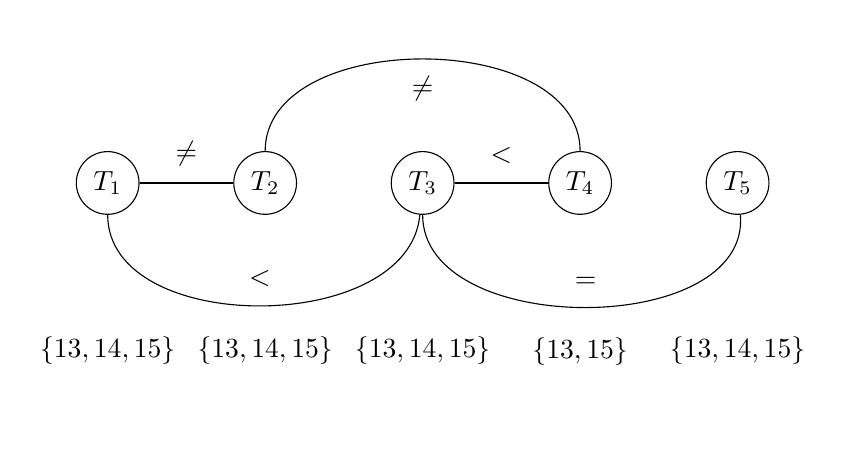
\begin{tikzpicture}[node distance=2cm, every node/.style={circle, draw}]
            \node (A) {$T_1$};
            \node (B) [right of =A] {$T_2$};
            \node (C) [right of =B] {$T_3$};
            \node (D) [right of =C] {$T_4$};
            \node (E) [right of =D] {$T_5$};

            \node[below=7mm of A, draw=none] {$\{13,14,15\}$};
            \node[below=7mm of B, draw=none] {$\{13,14,15\}$};
            \node[below=7mm of C, draw=none] {$\{13,14,15\}$};
            \node[below=9.5mm of D, draw=none] {$\{13,15\}$};
            \node[below=7mm of E, draw=none] {$\{13,14,15\}$};
            
            \draw (A) -- (B) node[midway, above, draw=none] {$\neq$};;
            \draw (C) -- (D) node[midway, above, draw=none] {$<$};;
            \path (A) edge [out=-90,in=-95] node[above, draw=none] {$<$} (C);
            \draw (C) edge [out=-90,in=-85] node[above, draw=none] {$=$} (E);
            \draw (B) edge [out=90,in=90] node[below, draw=none] {$\neq$} (D);
        \end{tikzpicture}
        \item Arc-consistent Graph after constraint propogation
         
        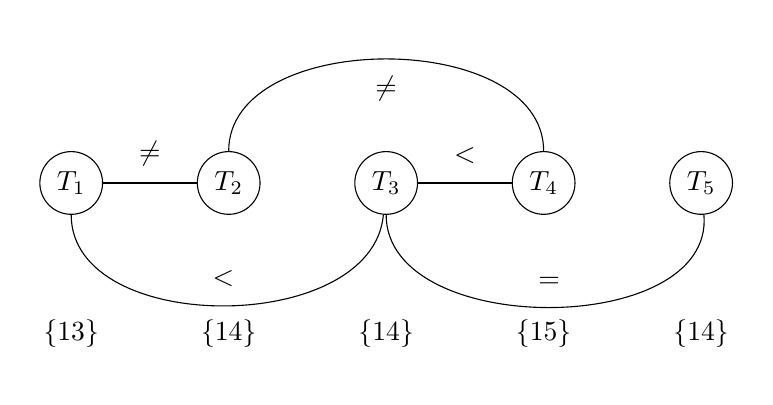
\begin{tikzpicture}[node distance=2cm, every node/.style={circle, draw}]
            \node (A) {$T_1$};
            \node (B) [right of =A] {$T_2$};
            \node (C) [right of =B] {$T_3$};
            \node (D) [right of =C] {$T_4$};
            \node (E) [right of =D] {$T_5$};

            \node[below=9.5mm of A, draw=none] {$\{13\}$};
            \node[below=9.5mm of B, draw=none] {$\{14\}$};
            \node[below=9.5mm of C, draw=none] {$\{14\}$};
            \node[below=9.5mm of D, draw=none] {$\{15\}$};
            \node[below=9.5mm of E, draw=none] {$\{14\}$};
            
            \draw (A) -- (B) node[midway, above, draw=none] {$\neq$};;
            \draw (C) -- (D) node[midway, above, draw=none] {$<$};;
            \path (A) edge [out=-90,in=-95] node[above, draw=none] {$<$} (C);
            \draw (C) edge [out=-90,in=-85] node[above, draw=none] {$=$} (E);
            \draw (B) edge [out=90,in=90] node[below, draw=none] {$\neq$} (D);
        \end{tikzpicture}
        
        \item A solution to the CSP is $T_1=13, T_2=14, T_3=14, T_4=15, T_5=14$
        \item It is not true that for very element x in the domain of a varaible v after propogation that there exists a solution where $v=x$.
        The propogation algorithm ensures that every pair of nodes are arc-consistent both ways (local consistency if nodes are also consistent). However, local consistency does not guarantee global consistency
        An example of such a graph is the one shown in the lecture:
        
        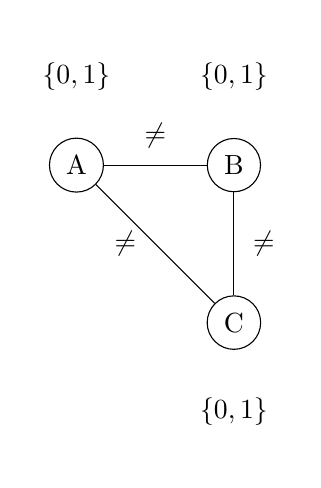
\begin{tikzpicture}[node distance=2cm, every node/.style={circle, draw}]
            \node (A) [circle, draw] {A};
            \node (B) [circle, draw, right of=A] {B};
            \node (C) [circle, draw, below of=B] {C};

            % Connect the nodes in a triangle
            \draw (A) -- node[midway, above, draw=none] {$\neq$} (B);
            \draw (B) -- node[midway, right, draw=none] {$\neq$} (C);
            \draw (C) -- node[midway, left, draw=none] {$\neq$} (A);

            % Add labels for the domain
            \draw (A) node [above, yshift=0.5cm,draw=none] {$\{0, 1\}$};
            \draw (B) node [above, yshift=0.5cm,draw=none] {$\{0, 1\}$};
            \draw (C) node [below, yshift=-0.5cm,draw=none] {$\{0, 1\}$};

        \end{tikzpicture}

        All the nodes are consistent and also consistent with respect to their neighbours but there is not solution, showing by conuterexample that there could still be elements left in the domain of a variable that are not in any solution.
    \end{enumerate}
\end{document}




%comm